%%%%%%%%%%%%%%%%%%%%%%%%%%%%%%%%%%%%%%%%%%%%%%%%%%%%%%%%%%%%
%  Unified EIT Model — UMN Beamer style
%  Local Income Taxes and Residential Sorting
%%%%%%%%%%%%%%%%%%%%%%%%%%%%%%%%%%%%%%%%%%%%%%%%%%%%%%%%%%%%

\documentclass[xcolor = x11names, compress, aspectratio = 169]{beamer}
\setbeamercovered{transparent}

%%%%%%%%%%%%%%%%  Dependencies %%%%%%%%%%%%%%%%%%%%%%%
\usepackage{graphicx}
\usepackage{booktabs}
\usepackage{textgreek}
\usepackage[round]{natbib}
\usepackage{colortbl}
\usepackage{amsmath}
\usepackage{amssymb}
\usepackage{multirow}
\usepackage{hyperref}
\usepackage{bm}

\usefonttheme[onlymath]{serif}
\beamertemplatenavigationsymbolsempty

%% UMN brand colors
\xdefinecolor{GopherMaroon}{HTML}{7A0019}
\xdefinecolor{GopherGold}{HTML}{FFCC33}
\xdefinecolor{GopherLightGold}{HTML}{FFDE7A}
\xdefinecolor{GopherDarkMaroon}{HTML}{5B0013}
%% Utility colors
\definecolor{ForestGreen}{RGB}{34,139,34}
\definecolor{DarkGray}{RGB}{100,100,100}

%%%%%%%%%%%%%%%% Beamer Layout %%%%%%%%%%%%%%%%%%%%%%
\useoutertheme[subsection = false, shadow]{miniframes}
\useinnertheme{default}
\usefonttheme{structureitalicserif}
\usepackage{palatino}
\setbeamerfont{title like}{shape = \scshape}
\setbeamerfont{frametitle}{shape = \scshape}

\setbeamercolor*{lower separation line head}{bg = GopherMaroon}
\setbeamercolor*{normal text}{fg = black, bg = white}
\setbeamercolor*{alerted text}{fg = GopherDarkMaroon}
\setbeamercolor*{example text}{fg = black}
\setbeamercolor*{structure}{fg = GopherDarkMaroon}

\setbeamercolor*{palette tertiary}{fg = GopherMaroon, bg = black!10}
\setbeamercolor*{palette quaternary}{fg = black, bg = black!10}

%% Footer: Hockert | Local Income Taxes | date + page number
\setbeamertemplate{footline}
{
    \leavevmode %
    \hbox{%
        \begin{beamercolorbox}[wd = .333333\paperwidth, ht = 2.25ex, dp = 1ex, center]{Author Footer} %
            Hockert
        \end{beamercolorbox}
        %
        \begin{beamercolorbox}[wd = .333333\paperwidth, ht = 2.25ex, dp = 1ex, center]{Title Footer} %
            Local Income Taxes \& Residential Sorting
        \end{beamercolorbox}
        %
        \begin{beamercolorbox}[wd = .333333\paperwidth, ht = 2.25ex, dp = 1ex, right]{Date Footer} %
            \usebeamerfont{Date Footer}\today \hspace*{2em}
            \insertframenumber{} / \inserttotalframenumber\hspace*{2ex}
        \end{beamercolorbox}}
        %
        \vskip0pt %
    }

\hypersetup{
    colorlinks,
    citecolor = GopherMaroon,
    linkcolor = black
}

\graphicspath{{../figures/}}

%%%%%%%%%%%%%%%%%%%%%%%%%%%%%%%%%%%%%%%%%%%%%%%%%%

\begin{document}

%%%%%%%%%%%%%%%%%%%%%%%%%%%%%%%%%%%%%%%%%%%%%%%%%%%%%%
%                Title Frame
%%%%%%%%%%%%%%%%%%%%%%%%%%%%%%%%%%%%%%%%%%%%%%%%%%%%%%

\begin{frame}
    \fontfamily{cmr}
    \title{Local Income Taxes and Residential Sorting \\
    \large A Unified Binding-State Decomposition}
    \author[Hockert]{
        Matthew Hockert$^\dagger$
    }
    \date{
        \small{\textit{\today}}
    }
    \institute[\textit{UMN}]{
        $^\dagger$\textit{Department of Applied Economics, \\
        University of Minnesota}
    }
    \titlepage
\end{frame}

%%%%%%%%%%%%%%%%%%%%%%%%%%%%%%%%%%%%%%%%%%%%%%%%%%%%%%
\section{Introduction}
%%%%%%%%%%%%%%%%%%%%%%%%%%%%%%%%%%%%%%%%%%%%%%%%%%%%%%

    %
    \begin{frame}
    \fontfamily{cmr}
    \frametitle{Question}
        \begin{itemize}\setlength{\itemsep}{0.15cm}
            \item When a Pennsylvania municipality changes its
            earned-income-tax rate, do workers \emph{sort} ---
            relocating residence or workplace?
            \item Three margins of response, all observable in LODES
            origin-destination data:
            \begin{itemize}\setlength{\itemsep}{0.05cm}
                \item \textbf{Live-and-work} workers: residents employed locally.
                \item \textbf{In-commuters}: nonresidents employed in the muni.
                \item \textbf{Out-commuters}: residents employed elsewhere.
            \end{itemize}
            \item Empirical challenge: the bill is piecewise
            $T = \max(\tau^{\text{home}},\, \tau^{\text{nr,work}})$.
            A rate change only \emph{moves the bill} when its side binds.
        \end{itemize}
    \end{frame}
    %

    %
    \begin{frame}
    \fontfamily{cmr}
    \frametitle{Roadmap}
        \begin{itemize}\setlength{\itemsep}{0.15cm}
            \item \textbf{Question:} Do PA EIT rate changes cause residential / job sorting?
            \item \textbf{Data:} LODES OD (2002--2019, PA) + DCED EIT panel + AFR fiscal panel.
            \item \textbf{Methods:} One muni $\times$ year panel; both
            $\Delta\tau^{\text{res}}$ and $\Delta\tau^{\text{nr}}$ in the same regression;
            decomposed by direction $\times$ binding state. Five estimators.
            \item \textbf{This deck:} Setup $\to$ cell counts $\to$ headline
            results $\to$ triangulation $\to$ event studies $\to$ placebo + robustness.
        \end{itemize}
    \end{frame}
    %

%%%%%%%%%%%%%%%%%%%%%%%%%%%%%%%%%%%%%%%%%%%%%%%%%%%%%%
\section{Background}
%%%%%%%%%%%%%%%%%%%%%%%%%%%%%%%%%%%%%%%%%%%%%%%%%%%%%%

    %
    \begin{frame}
    \fontfamily{cmr}
    \frametitle{Institutional Setting (PA EIT, post-Act 32)}
        \footnotesize
        For a PA resident working outside Philadelphia:
        \[
            T_{ij} = \max\!\bigl(\tau^{\text{res}}_j + \tau^{\text{SD}}_j,\; \tau^{\text{nr}}_i\bigr).
        \]
        Liability allocation: work muni collects up to its nonres rate;
        home muni + SD collect any residual.
        \medskip

        \begin{itemize}\setlength{\itemsep}{0.10cm}
            \item \textbf{Act 32 (2008 / effective 2012)} standardized
            employer withholding, residency certification, and consolidated
            tax-collection districts. Statutory rates were unchanged ---
            the change was administrative.
            \item \textbf{Empirical implication.} Pre-Act-32, the same
            statutory rate was weakly enforced. Post-Act-32, the binding
            rule above actually moves the bill.
            \item \textbf{Sample.} 2002--2019 (avoid COVID).
        \end{itemize}
    \end{frame}
    %

    %
    \begin{frame}
    \fontfamily{cmr}
    \frametitle{Data}
        \footnotesize
        \begin{itemize}\setlength{\itemsep}{0.10cm}
            \item \textbf{LODES OD} (2002--2019, PA): block-level
            origin-destination flows aggregated to PA county subdivisions
            (cousubs) via TIGER 2020 block centroid. Recovers all
            2{,}561 PA cousubs (vs 1{,}479 under the prior tract-centroid join).
            \item \textbf{DCED EIT panel}: muni $\times$ year resident,
            school district, and nonresident rates. Reparsed XLS to
            recover SD identifiers. Nonres rate has reporting gaps
            (handled via three sample variants).
            \item \textbf{DCED AFR}: muni fiscal panel for controls
            (log spending: police, streets, debt, state aid; revenue
            shares: EIT, real estate, intergov).
            \item \textbf{Sample}: $\sim$2{,}500 cousubs $\times$ 18 years.
        \end{itemize}
    \end{frame}
    %

%%%%%%%%%%%%%%%%%%%%%%%%%%%%%%%%%%%%%%%%%%%%%%%%%%%%%%
\section{Methods}
%%%%%%%%%%%%%%%%%%%%%%%%%%%%%%%%%%%%%%%%%%%%%%%%%%%%%%

    %
    \begin{frame}
    \fontfamily{cmr}
    \frametitle{Setup: One Panel, Three Treatments}
        \footnotesize
        \textbf{Unit} $i$: a PA cousub. \textbf{Time} $t$: year.
        One row per $(i,t)$.
        \medskip

        \textbf{Outcomes per row} (eight; covered simultaneously):
        \begin{itemize}\setlength{\itemsep}{0.02cm}\scriptsize
            \item \texttt{log\_live\_and\_work}, \texttt{log\_in\_commuters},
            \texttt{log\_out\_commuters}
            \item \texttt{log\_total\_jobs}, \texttt{log\_total\_residents}
            \item \texttt{share\_live\_in}, \texttt{share\_nonres},
            \texttt{share\_work\_outside}
        \end{itemize}
        \medskip

        \textbf{Three treatments per row}, each separately decomposed by cells:
        \begin{itemize}\setlength{\itemsep}{0.02cm}\scriptsize
            \item $\Delta\tau^{\text{muni}}_{it}$: cumulative muni resident-rate change.
            \item $\Delta\tau^{\text{SD}}_{it}$: cumulative school-district rate change.
            \item $\Delta\tau^{\text{nr}}_{it}$: cumulative muni nonresident-rate change.
        \end{itemize}
        \medskip

        \textbf{Per-row binding state}:
        $\text{home\_binds}_{it} = \mathbf{1}\{\tau^{\text{home}}_{it} > \tau^{\text{nr}}_{it}\}$
        where $\tau^{\text{home}} = \tau^{\text{muni}} + \tau^{\text{SD}}$.
        Cells classified separately for each treatment using its own first event.
    \end{frame}
    %

    %
    \begin{frame}
    \fontfamily{cmr}
    \frametitle{Cell Classification (per side, fixed at first event)}
        \footnotesize
        Each muni gets one cell label on each side, based on the
        binding state \emph{just before} vs \emph{just after} its first event.
        \medskip
        \scriptsize
        \renewcommand{\arraystretch}{1.20}
        \setlength{\tabcolsep}{6pt}
        \begin{tabular}{lll}
            \toprule
            Cell & Direction & Binding transition \\
            \midrule
            \textcolor{GopherMaroon}{\textbf{Inc-bind}}     & Up   & binding pre and post (bill $\uparrow$ by full $\Delta\tau$) \\
            \textcolor{GopherMaroon!70}{\textbf{Inc-becomes}} & Up   & flips non-binding $\to$ binding (bill rises by $\tau_{\text{post}} - \tau^{\text{nr}}$) \\
            \textcolor{DarkGray}{\textbf{Inc-nobind}}        & Up   & non-binding throughout (\textbf{bill unchanged} --- placebo) \\
            \textcolor{GopherDarkMaroon}{\textbf{Dec-bind}}  & Down & binding pre and post (bill $\downarrow$ by full $\Delta\tau$) \\
            \textbf{Dec-becomes-non}                          & Down & flips binding $\to$ non-binding \\
            \textcolor{DarkGray}{\textbf{Dec-nobind}}         & Down & non-binding throughout (\textbf{bill unchanged} --- placebo) \\
            NC                                                & ---  & never-changed (control) \\
            \bottomrule
        \end{tabular}
        \medskip
        \footnotesize
        Institutional rule predicts |Inc-bind| $>$ |Inc-becomes| $>$ |Inc-nobind|
        (= 0). Inc-nobind and Dec-nobind are \textbf{predicted-null
        placebos within the design.}
    \end{frame}
    %

    %
    \begin{frame}
    \fontfamily{cmr}
    \frametitle{Estimating Equation}
        \scriptsize
        For outcome $Y$ and estimator $E$:
        \begin{equation*}
        \begin{split}
        Y_{it} = \alpha_i + \gamma_t
          &+ \sum_{k}\beta^{\text{muni}}_k\,\Delta\tau^{\text{muni}}_{it}\cdot\mathbf{1}\{\text{cell}^{\text{muni}}_i=k\} \\
          &+ \sum_{k}\beta^{\text{SD}}_k\,\Delta\tau^{\text{SD}}_{it}\cdot\mathbf{1}\{\text{cell}^{\text{SD}}_i=k\} \\
          &+ \sum_{k}\beta^{\text{nr}}_k\,\Delta\tau^{\text{nr}}_{it}\cdot\mathbf{1}\{\text{cell}^{\text{nr}}_i=k\}
          + \mathbf{X}'_{it}\phi + \varepsilon_{it}
        \end{split}
        \end{equation*}
        \footnotesize
        \begin{itemize}\setlength{\itemsep}{0.04cm}
            \item Both treatments and their cell decompositions enter the
            \emph{same} regression. No OD flows; no pair panel.
            \item Reference cell on each side: NC (never-changed).
            \item $\mathbf{X}_{it}$: log spending on police, streets,
            debt, state aid; revenue shares (EIT, RE).
            \item Fixed effects: muni $\alpha_i$, year $\gamma_t$.
            SE clustered at muni.
        \end{itemize}
        \medskip

        \textbf{Five estimators.} Q2 TWFE pooled $\to$ single-event TWFE
        ($\le 2$ events per side) $\to$ stacked DiD binary
        (cell $\times$ post) $\to$
        \alert{stacked DiD continuous (cell $\times \Delta\tau$, headline)}
        $\to$ DCDH (per cell, continuous).
    \end{frame}
    %

    %
    \begin{frame}
    \fontfamily{cmr}
    \frametitle{Three Sample Variants for Missing Nonres Rates}
        \footnotesize
        DCED's nonres-rate reporting is patchy pre-Act-32 ($\sim$55\%
        coverage) and incomplete post ($\sim$72--80\%). All else equal,
        we run three samples:
        \medskip
        \scriptsize
        \renewcommand{\arraystretch}{1.20}
        \setlength{\tabcolsep}{8pt}
        \begin{tabular}{ll}
            \toprule
            Sample & Treatment of NA \texttt{muni\_nonres\_eit} \\
            \midrule
            \textbf{strict} & Drop muni-years with NA nonres rate. \\
            \textbf{filled} & Impute \texttt{nonres = resident\_eit} when NA (statute-anchored). \\
            \textbf{drop}   & Keep all years; drop NA at regression time per outcome. \\
            \bottomrule
        \end{tabular}
        \medskip
        \footnotesize
        \textbf{Headline tables}: \texttt{drop} sample (largest N).
        \texttt{filled} and \texttt{strict} reported as robustness.
    \end{frame}
    %

%%%%%%%%%%%%%%%%%%%%%%%%%%%%%%%%%%%%%%%%%%%%%%%%%%%%%%
\section{Results}
%%%%%%%%%%%%%%%%%%%%%%%%%%%%%%%%%%%%%%%%%%%%%%%%%%%%%%

    %
    \begin{frame}
    \fontfamily{cmr}
    \frametitle{Cell Counts (drop sample, unique munis)}
        \centering
        \footnotesize
        \renewcommand{\arraystretch}{1.20}
        \setlength{\tabcolsep}{6pt}
        \begin{tabular}{lcccccccc}
            \toprule
            Treatment & Inc-bind & Inc-becomes & Inc-nobind & Dec-bind & Dec-becomes & Dec-nobind & NC \\
            \midrule
            Muni resident          & 40  & 58  & 26 & 11 & 4 & 15  & 2{,}406 \\
            School district (SD)   & 75  & 197 & 14 & 4  & 10 & ---  & 2{,}253 \\
            Muni nonresident       & 0   & 0   & 171 & 0  & 5 & 109 & 2{,}276 \\
            \bottomrule
        \end{tabular}
        \medskip
        \begin{itemize}\setlength{\itemsep}{0.04cm}\scriptsize
            \item Three treatments share the same binding indicator
            (home\_stack vs nonres) and same outcome panel.
            \item \textbf{Muni and SD events differ in count and timing}:
            SD events are more common, especially Inc-becomes (197 vs 58 muni).
            \item \textbf{Nonres-side binding decomposition collapses}: in PA,
            $\tau^{\text{nr}}$ almost never exceeds home\_stack at the
            muni-self-pair level (Philadelphia is the rare exception, excluded).
            Effectively one Inc cell + two Dec cells.
        \end{itemize}
    \end{frame}
    %

    %
    \begin{frame}
    \fontfamily{cmr}
    \frametitle{Muni Resident Rate: Stacked Continuous, Drop Sample}
        \centering
        \scriptsize
        \renewcommand{\arraystretch}{1.10}
        \setlength{\tabcolsep}{4pt}
        \begin{tabular}{lcccccc}
            \toprule
            & Inc-bind & Inc-becomes & Inc-nobind & Dec-bind & Dec-becomes & Dec-nobind \\
            & ($n$=40) & ($n$=58) & \emph{placebo} ($n$=26) & ($n$=11) & ($n$=4) & \emph{placebo} ($n$=15) \\
            \midrule
            log(live\_and\_work)    & $\bm{-0.283^{***}}$ & $\bm{-0.142^{***}}$ & $-0.079$       & $-0.283$       & $-0.641$       & $-0.139$ \\
            log(in\_commuters)      & $-0.076$            & $\bm{-0.154^{***}}$ & $-0.077$       & $+0.018$       & $+0.363^{***}$ & $-0.125$ \\
            log(out\_commuters)     & $\bm{-0.078^{*}}$   & $-0.029$            & $+0.136$       & $+0.167^{*}$   & $-0.798$       & $-0.052$ \\
            log(total\_jobs)        & $-0.125$            & $\bm{-0.152^{***}}$ & $-0.084$       & $+0.038$       & $+0.250^{*}$   & $-0.141$ \\
            log(total\_residents)   & $\bm{-0.117^{***}}$ & $\bm{-0.056^{**}}$  & $+0.067$       & $+0.169$       & $-0.847$       & $-0.053$ \\
            share\_live\_in         & $\bm{-0.039^{***}}$ & $+0.000$            & $-0.007$       & $+0.017$       & $-0.099^{*}$   & $-0.008$ \\
            share\_work\_outside    & $\bm{+0.033^{**}}$  & $\bm{+0.020^{***}}$ & $+0.053^{***}$ & $-0.002$       & $+0.036^{***}$ & $+0.001$ \\
            \bottomrule
        \end{tabular}
        \vspace{0.10cm}
        \begin{minipage}{0.95\textwidth}
            \tiny \textit{Notes:} Stacked-continuous DiD ($\pm$5-yr window).
            $\Delta\tau^{\text{muni}}$, $\Delta\tau^{\text{SD}}$, and
            $\Delta\tau^{\text{nr}}$ cell interactions in the same regression
            (only muni cells shown here; SD on next slide).
            Cluster-robust SEs by muni.
            $^{*}p<0.10$, $^{**}p<0.05$, $^{***}p<0.01$.
        \end{minipage}
    \end{frame}
    %

    %
    \begin{frame}
    \fontfamily{cmr}
    \frametitle{School District Rate: Stacked Continuous, Drop Sample}
        \centering
        \scriptsize
        \renewcommand{\arraystretch}{1.10}
        \setlength{\tabcolsep}{4pt}
        \begin{tabular}{lccccc}
            \toprule
            & Inc-bind & Inc-becomes & Inc-nobind & Dec-bind & Dec-becomes \\
            & ($n$=75) & ($n$=197) & ($n$=14) & ($n$=4) & ($n$=10) \\
            \midrule
            log(live\_and\_work)    & $+0.058$         & $+0.229$       & ---            & $\bm{-0.669^{***}}$ & $-0.212^{*}$ \\
            log(in\_commuters)      & $+0.099^{*}$     & $+0.028$       & ---            & $\bm{-0.085^{***}}$ & $-0.073$ \\
            log(out\_commuters)     & $+0.001$         & $+0.028$       & ---            & $\bm{+0.330^{***}}$ & $-0.030$ \\
            log(total\_jobs)        & $+0.076$         & $+0.030$       & ---            & $\bm{-0.113^{***}}$ & $-0.074$ \\
            log(total\_residents)   & $-0.010$         & $-0.011$       & ---            & $\bm{+0.322^{***}}$ & $-0.034$ \\
            share\_live\_in         & $\bm{-0.017^{***}}$ & $+0.001$    & ---            & $\bm{-0.027^{***}}$ & $-0.001$ \\
            share\_work\_outside    & $+0.008^{*}$     & $+0.021$       & ---            & $\bm{+0.007^{***}}$ & $+0.003$ \\
            \bottomrule
        \end{tabular}
        \vspace{0.10cm}
        \begin{minipage}{0.95\textwidth}
            \tiny \textit{Notes:} SD-rate cells are largely null. Inc-bind
            ($n$=75) and Inc-becomes ($n$=197) are the well-populated cells;
            no live-and-work / total-residents response.
            Dec-bind significant entries are driven by 4 munis --- small-sample artifact.
            Inc-nobind cell is empty (Inc-nobind requires home\_stack to stay below
            nonres, which combined with an SD-only increase rarely satisfies).
            Same regression as previous slide.
        \end{minipage}
    \end{frame}
    %

    %
    \begin{frame}
    \fontfamily{cmr}
    \frametitle{Reading: Muni Rate Drives Sorting; SD Does Not}
        \footnotesize
        \begin{itemize}\setlength{\itemsep}{0.10cm}
            \item Within the binding decomposition, the \textbf{muni-rate
            Inc-bind cell} produces $-0.283^{***}$ on log(live\_and\_work);
            the \textbf{SD-rate Inc-bind cell} produces $+0.058$ (insig).
            \item \textbf{SD changes don't move residents}, even when
            they flip the binding state. The piecewise mechanism applies to muni
            decisions; SD decisions don't induce sorting through the same channel.
            \item This validates the prior block-level-LODES finding (SD null)
            \emph{within} the new binding-decomposition design --- a stronger test.
            \item The current Q3 deck attributed all resident-side action to
            the resident rate without explicitly partialing out SD.
            Mode B confirms the muni-rate coefficient ($-0.283$) is
            essentially identical to the muni-only spec ($-0.290$) ---
            \textbf{SD doesn't confound}, it just doesn't sort.
        \end{itemize}
    \end{frame}
    %

    %
    \begin{frame}
    \fontfamily{cmr}
    \frametitle{Reading the Muni-Rate Cells}
        \footnotesize
        \textbf{Inc-bind} (muni rate up; bill rises by full $\Delta\tau^{\text{muni}}$):
        \begin{itemize}\setlength{\itemsep}{0.02cm}\scriptsize
            \item Live-and-work workers $\downarrow$ 28\%; total residents $\downarrow$ 12\%.
            \item Share commuting out $\uparrow$ +3.3pp.
            \item Cleanest evidence of residential sorting in the data.
        \end{itemize}

        \textbf{Inc-becomes} (muni rate up; bill newly starts moving):
        \begin{itemize}\setlength{\itemsep}{0.02cm}\scriptsize
            \item Smaller live-and-work effect ($-0.142$) --- bill rises
            by less than $\Delta\tau$ in this cell.
            \item In-commuters $\downarrow$ 15\%; total jobs $\downarrow$ 15\%.
        \end{itemize}

        \textbf{\textcolor{DarkGray}{Inc-nobind}} (muni rate up; bill never moves --- placebo):
        \begin{itemize}\setlength{\itemsep}{0.02cm}\scriptsize
            \item Null on every level outcome.
            \item \alert{Placebo passes.} Institutional rule, not generic
            confounding, identifies the response.
        \end{itemize}

        \textbf{Dec cells}: 11--26 munis combined; underpowered.
    \end{frame}
    %

    %
    \begin{frame}
    \fontfamily{cmr}
    \frametitle{Nonresident Side: Stacked Continuous, Drop Sample}
        \centering
        \scriptsize
        \renewcommand{\arraystretch}{1.15}
        \setlength{\tabcolsep}{8pt}
        \begin{tabular}{lccc}
            \toprule
            & Inc-nobind & Dec-becomes-non & Dec-nobind \\
            & ($n$=171) & ($n$=5) & ($n$=109) \\
            \midrule
            log(live\_and\_work)   & $-0.157$           & $-0.072^{**}$  & $-0.227$ \\
            log(in\_commuters)     & $\bm{-0.363^{**}}$ & $+0.070^{***}$ & $-0.326$ \\
            log(out\_commuters)    & $-0.025$           & $-0.061^{*}$   & $+0.010$ \\
            log(total\_jobs)       & $\bm{-0.362^{**}}$ & $+0.020$       & $-0.325$ \\
            log(total\_residents)  & $-0.031$           & $-0.079^{***}$ & $+0.001$ \\
            share\_nonres          & $-0.001$           & $+0.036^{***}$ & $-0.000$ \\
            \bottomrule
        \end{tabular}
        \vspace{0.10cm}

        \footnotesize
        A muni-nonres-rate increase pushes \emph{nonresident workers out}
        ($-36\%$); total jobs fall in tandem; \textbf{residents are unaffected}.
        \medskip\\
        Channels stay cleanly separated: nonres rate hits in-commuters;
        does not measurably affect the muni's own residents on either margin.
    \end{frame}
    %

    %
    \begin{frame}
    \fontfamily{cmr}
    \frametitle{Cross-Effects: Are the Channels Separated?}
        \centering
        \footnotesize
        \renewcommand{\arraystretch}{1.20}
        \setlength{\tabcolsep}{6pt}
        \begin{tabular}{lcc|cc|cc}
            \toprule
            & \multicolumn{2}{c|}{Muni-rate (Inc-bind)} & \multicolumn{2}{c|}{SD-rate (Inc-bind)} & \multicolumn{2}{c}{Nonres-rate (Inc-nobind)} \\
            Outcome & coef & sig & coef & sig & coef & sig \\
            \midrule
            log(live\_and\_work)   & $-0.283$ & $***$ & $+0.058$ & ---   & $-0.157$ & --- \\
            log(in\_commuters)     & $-0.076$ & ---   & $+0.099$ & $*$   & $-0.363$ & $**$ \\
            log(total\_residents)  & $-0.117$ & $***$ & $-0.010$ & ---   & $-0.031$ & --- \\
            log(out\_commuters)    & $-0.078$ & $*$   & $+0.001$ & ---   & $-0.025$ & --- \\
            \bottomrule
        \end{tabular}
        \medskip

        \footnotesize
        \begin{itemize}\setlength{\itemsep}{0.04cm}
            \item \textbf{Muni rate hike} $\to$ residents leave; SD doesn't move them; in-commuters mostly unaffected.
            \item \textbf{SD rate hike} $\to$ no significant resident response; small in-commuters bump (10\%) at $p<0.10$.
            \item \textbf{Nonres rate hike} $\to$ in-commuters leave; residents unaffected.
            \item Three rates, three populations: muni $\to$ residents; SD $\to$ no one;
            nonres $\to$ in-commuters.
        \end{itemize}
    \end{frame}
    %

    %
    \begin{frame}
    \fontfamily{cmr}
    \frametitle{Estimator Triangulation: log(live\_and\_work), Muni Inc Cells}
        \centering
        \footnotesize
        \renewcommand{\arraystretch}{1.20}
        \setlength{\tabcolsep}{8pt}
        \begin{tabular}{lccc}
            \toprule
            Estimator & Inc-bind & Inc-becomes & Inc-nobind (placebo) \\
            \midrule
            Q2 TWFE pooled                & $-0.238^{***}$       & $-0.154^{***}$       & $-0.089^{**}$ \\
            Single-event TWFE ($\le$2)    & $-0.157$             & $-0.201^{***}$       & $-0.078$ \\
            Stacked binary                & $-0.086^{*}$         & $-0.094^{**}$        & $-0.022$ \\
            \alert{Stacked continuous}    & \alert{$\bm{-0.283^{***}}$} & \alert{$\bm{-0.142^{***}}$} & $-0.079$ \\
            DCDH (effects=3 horizon)      & $-0.054$             & $-0.003$             & $-0.008$ \\
            \bottomrule
        \end{tabular}
        \medskip

        \footnotesize
        \begin{itemize}\setlength{\itemsep}{0.04cm}\scriptsize
            \item Muni Inc-bind: negative across every estimator; magnitude
            $-0.05$ (DCDH 3-yr horizon) to $-0.28$ (stacked continuous).
            \item Muni Inc-becomes: negative across every estimator with signal.
            \item \textbf{Muni Inc-nobind (placebo)}: tightly null across estimators;
            only Q2 TWFE pooled reaches 10\% --- the spec most contaminated
            by negative weighting.
        \end{itemize}
    \end{frame}
    %

    %
    \begin{frame}
    \fontfamily{cmr}
    \frametitle{Event Study: log(live\_and\_work), Inc Cells}
        \vfill
        \centering
        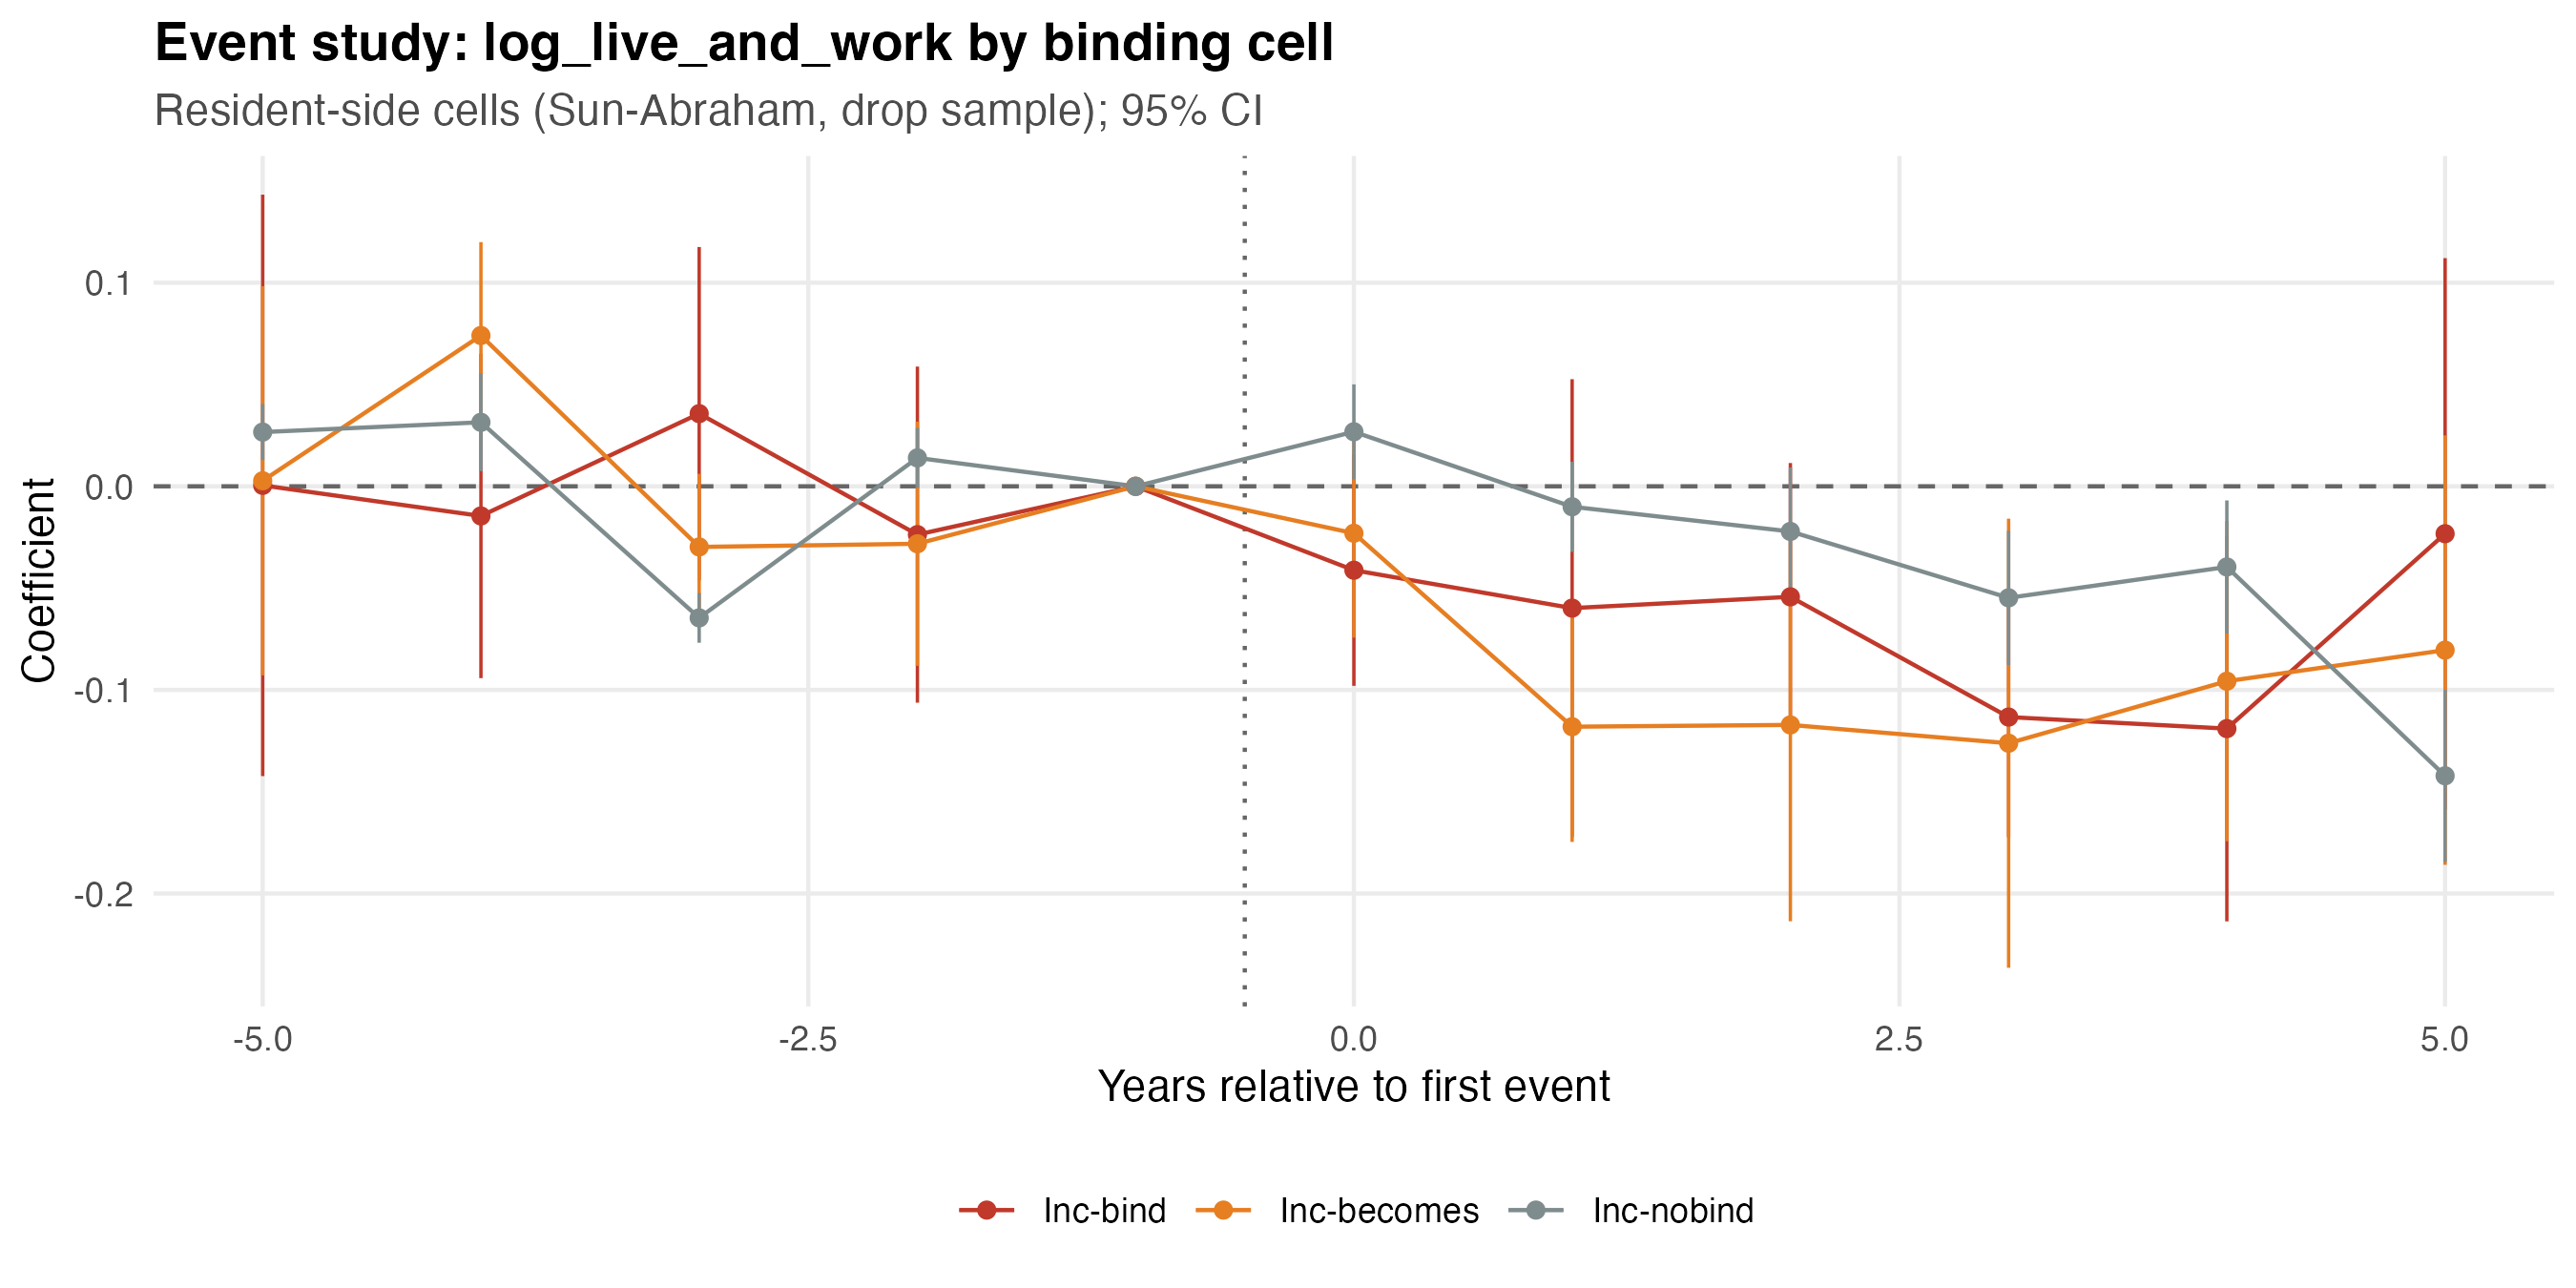
\includegraphics[width=0.85\textwidth]{unified_es_res_inc_log_live_and_work.png}
        \vfill
        \footnotesize
        Sun-Abraham. Resident-side Inc cells vs NC controls. Drop sample.
        Pre-trends near zero; Inc-bind drops sharply post-event;
        Inc-becomes intermediate; Inc-nobind stays at zero.
    \end{frame}
    %

    %
    \begin{frame}
    \fontfamily{cmr}
    \frametitle{Event Study: log(total\_residents), Inc Cells}
        \vfill
        \centering
        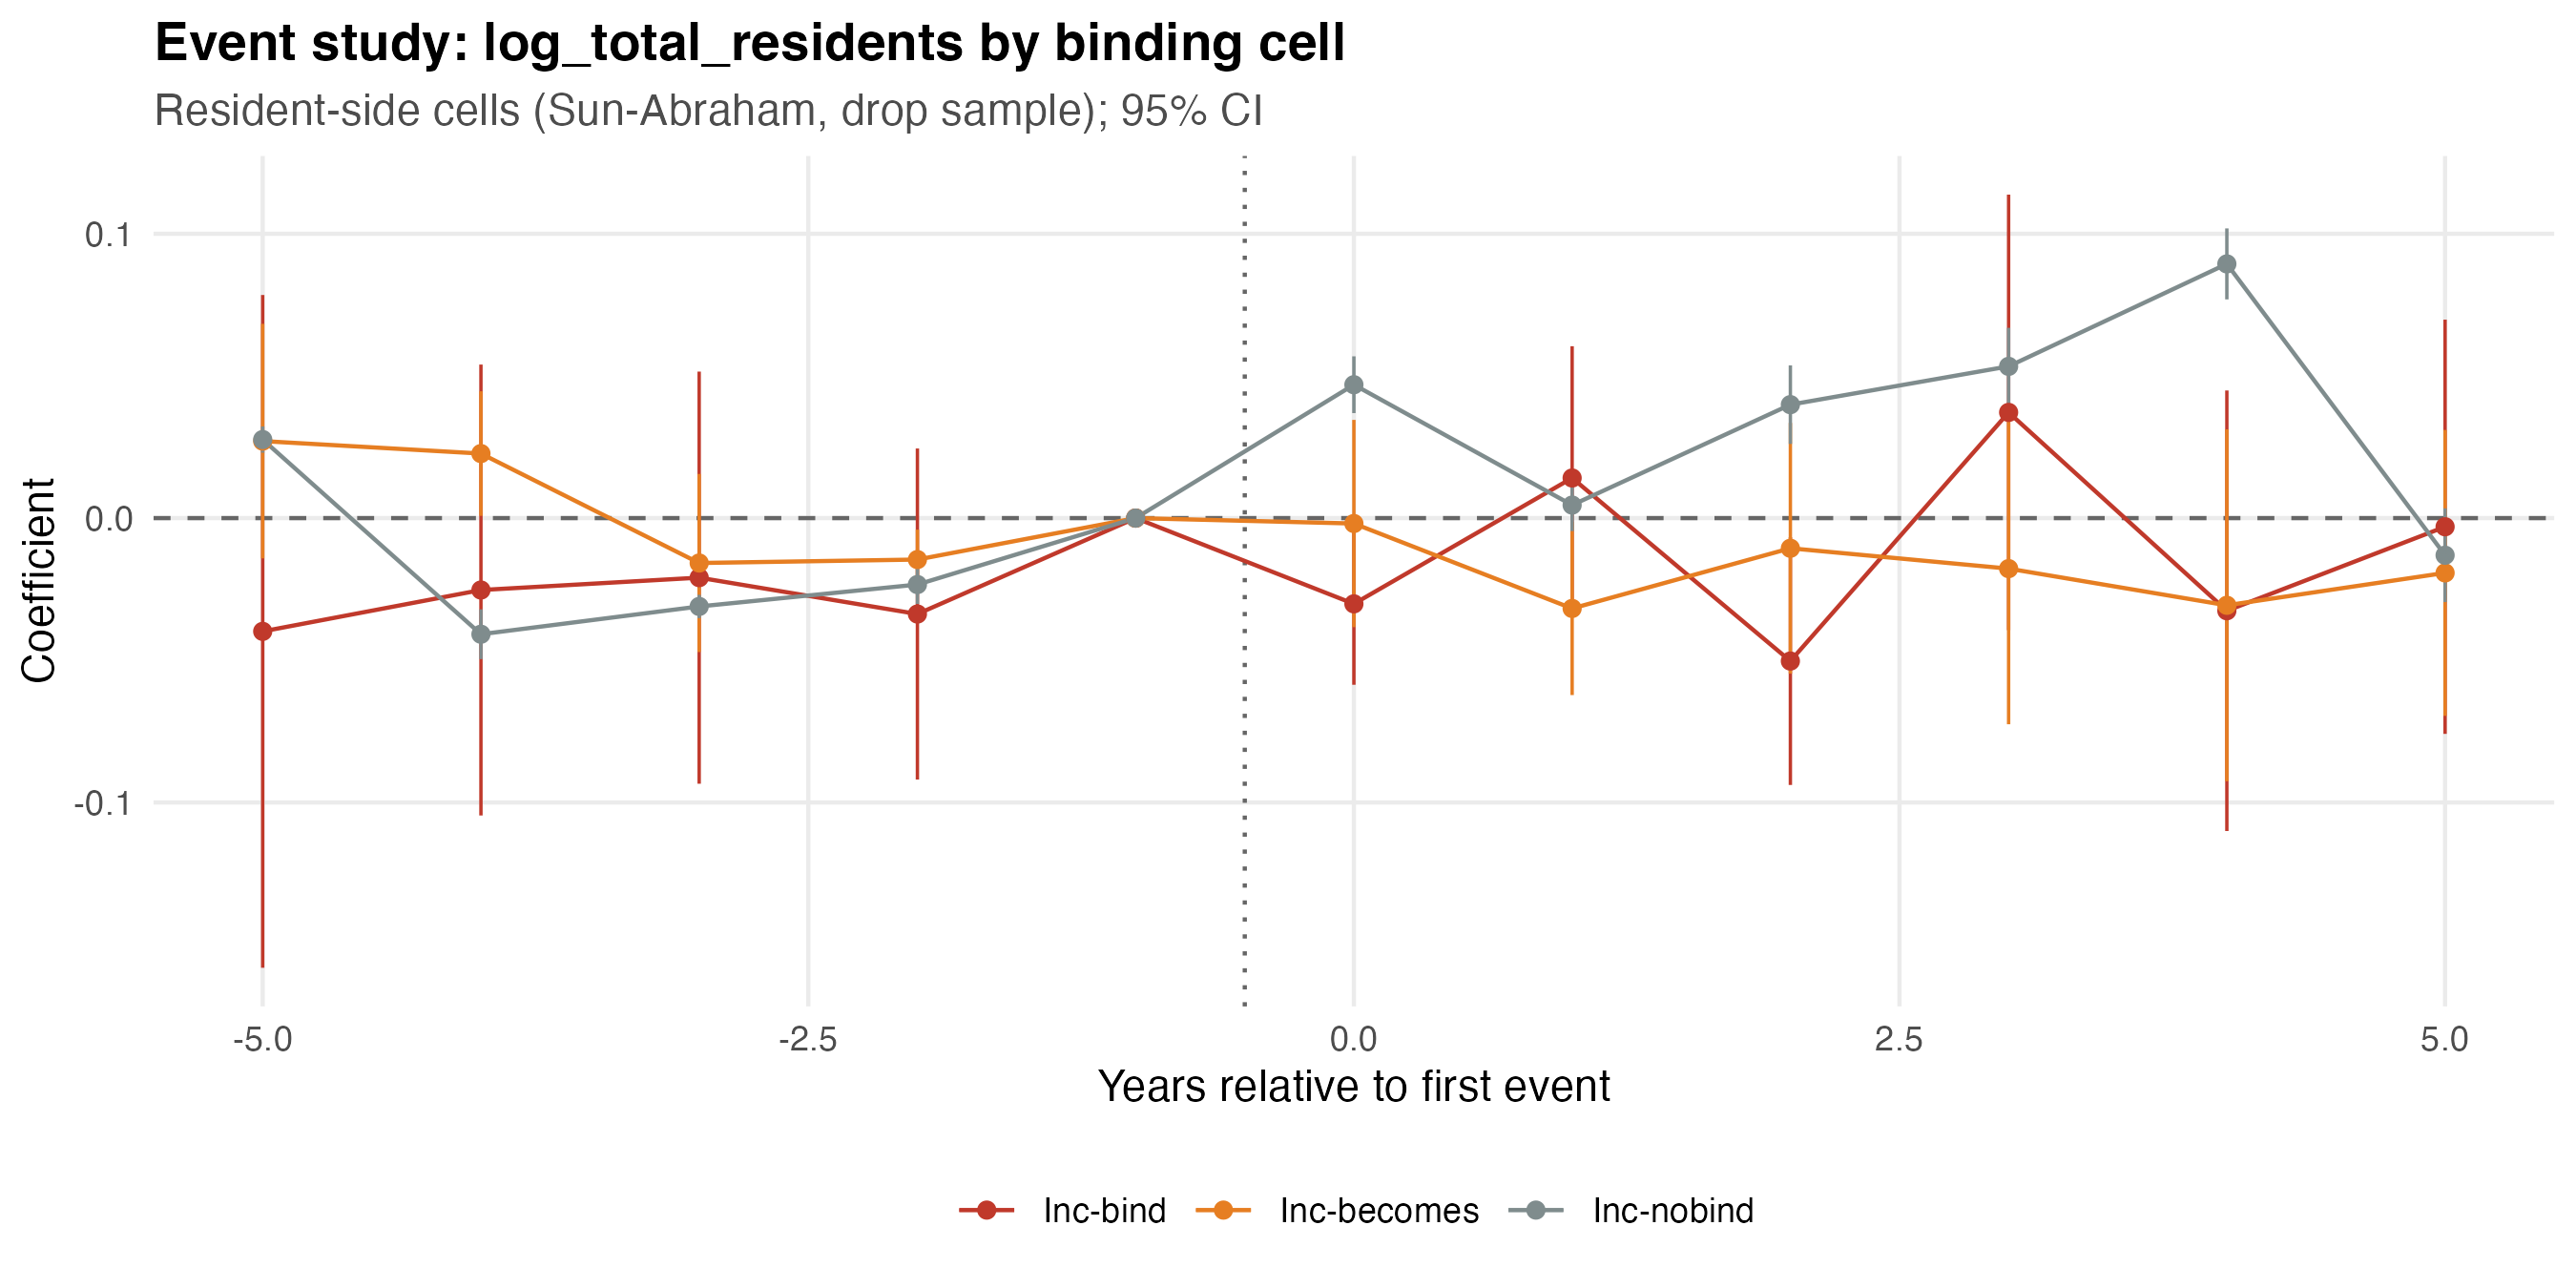
\includegraphics[width=0.85\textwidth]{unified_es_res_inc_log_total_residents.png}
        \vfill
        \footnotesize
        Total employed residents. Inc-bind: $\sim$10\% drop within 5 years.
        Inc-becomes: $\sim$5\%. Inc-nobind: flat.
    \end{frame}
    %

    %
    \begin{frame}
    \fontfamily{cmr}
    \frametitle{Event Study: share\_live\_in, Inc Cells}
        \vfill
        \centering
        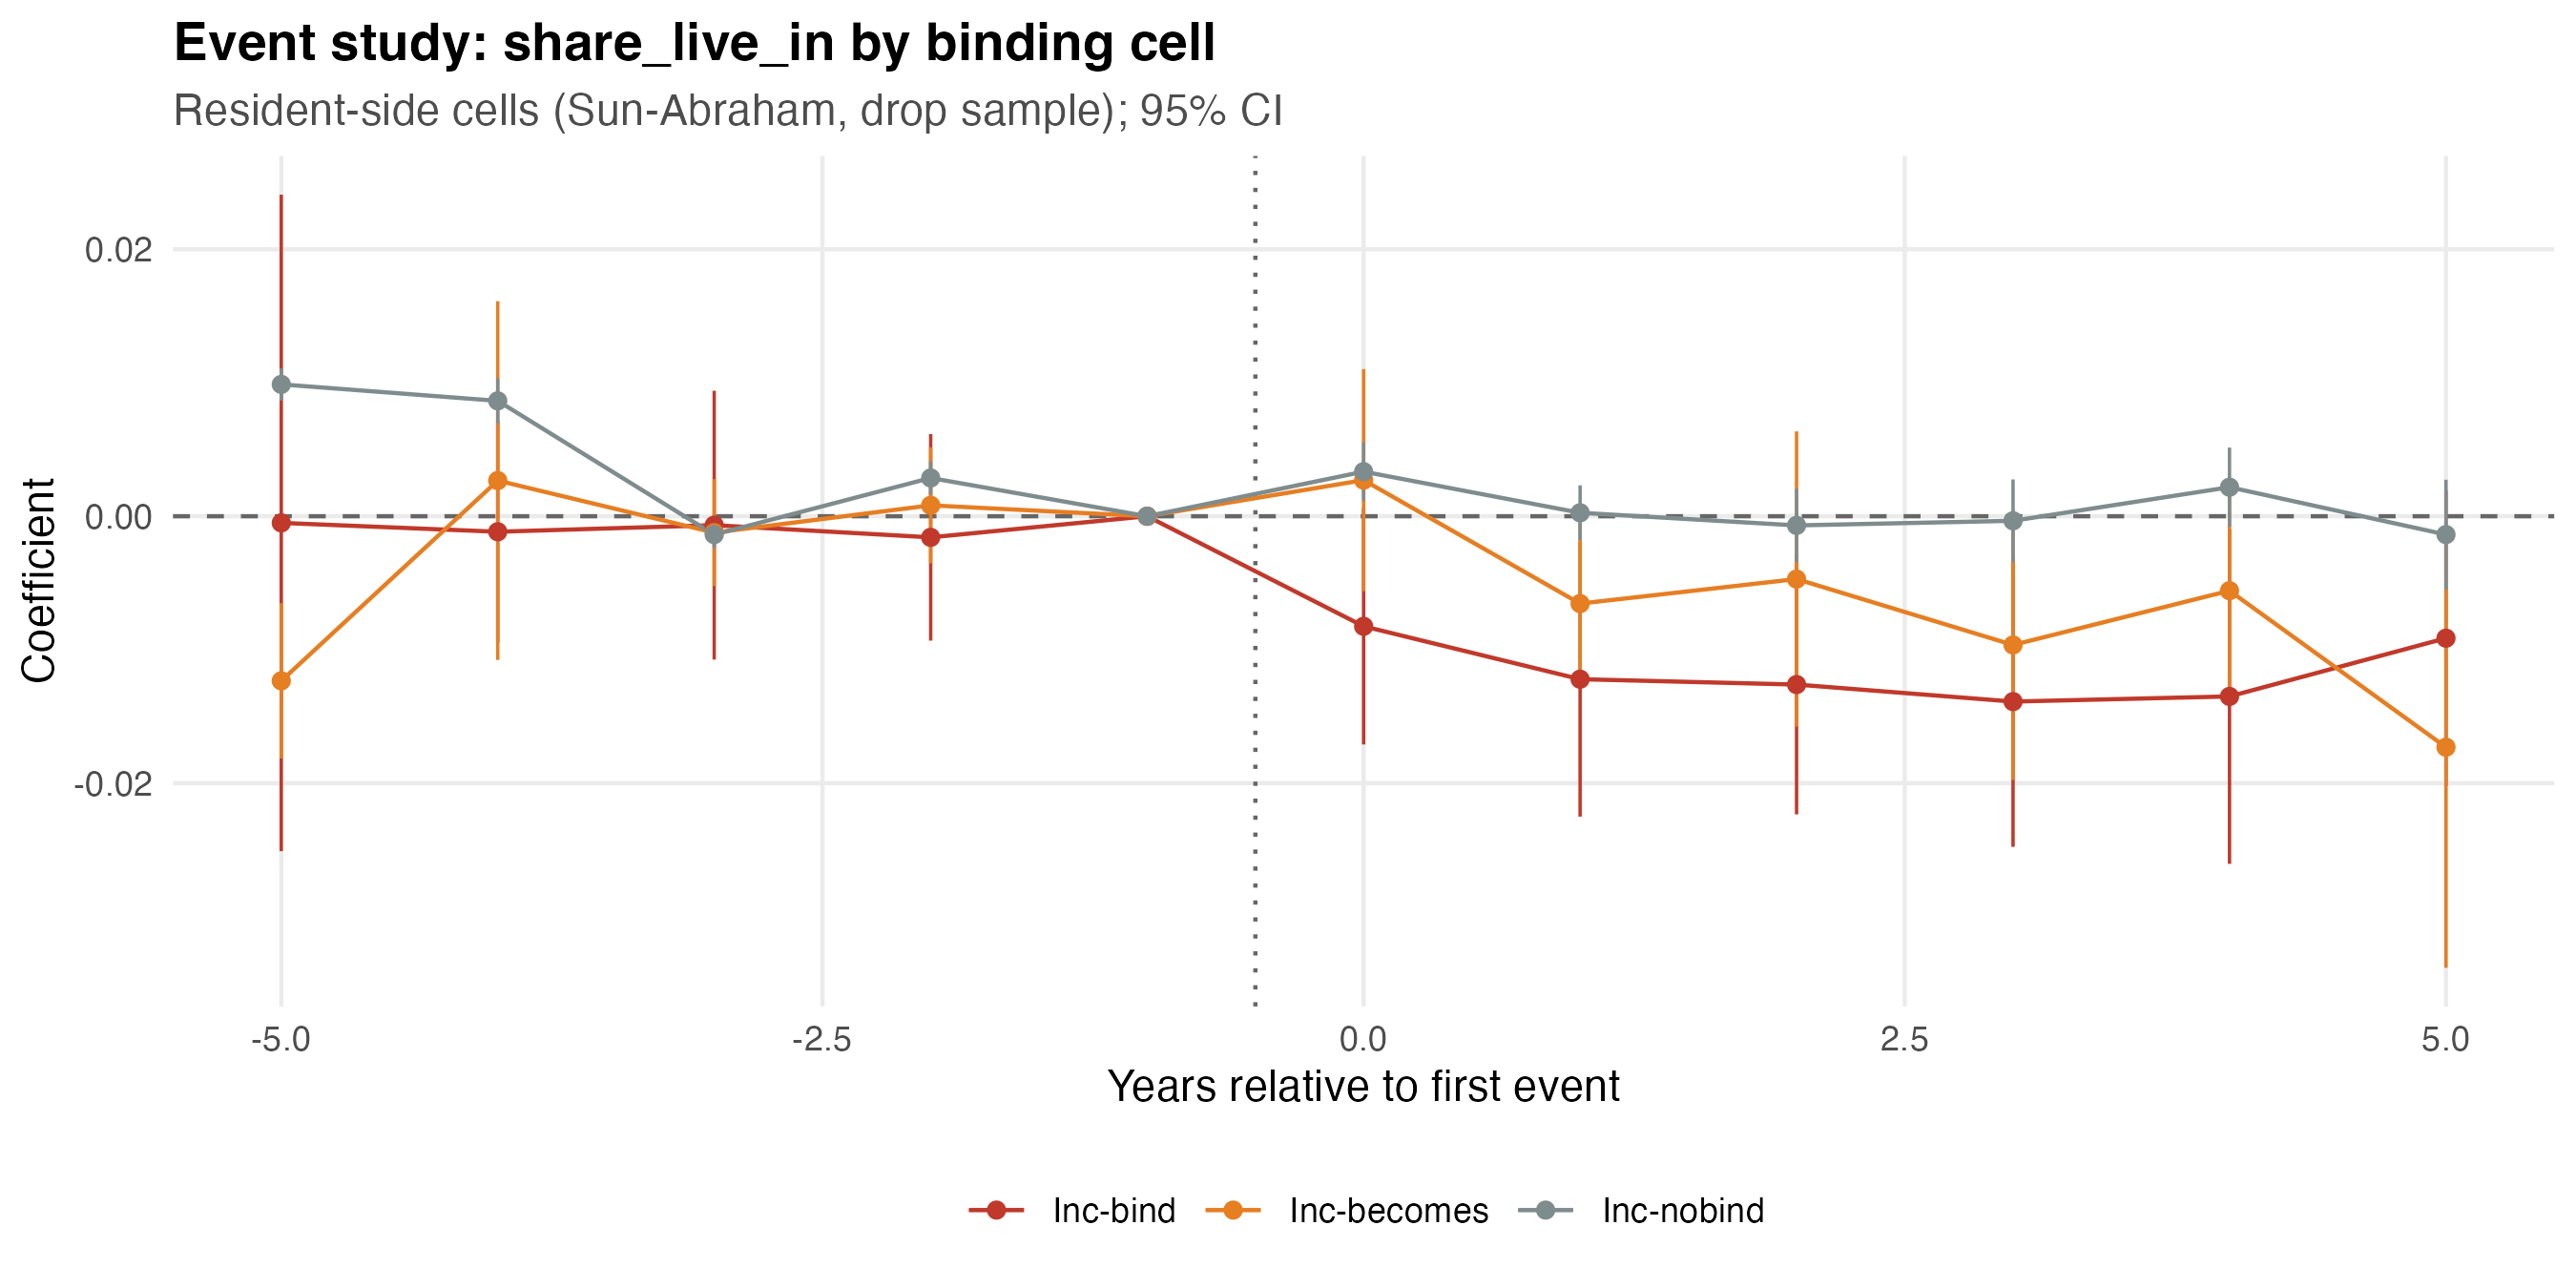
\includegraphics[width=0.85\textwidth]{unified_es_res_inc_share_live_in.png}
        \vfill
        \footnotesize
        Share of jobs filled by in-muni residents. Inc-bind: $-4$pp by year 5.
        Placebo cell flat.
    \end{frame}
    %

    %
    \begin{frame}
    \fontfamily{cmr}
    \frametitle{Event Study: share\_work\_outside, Inc Cells}
        \vfill
        \centering
        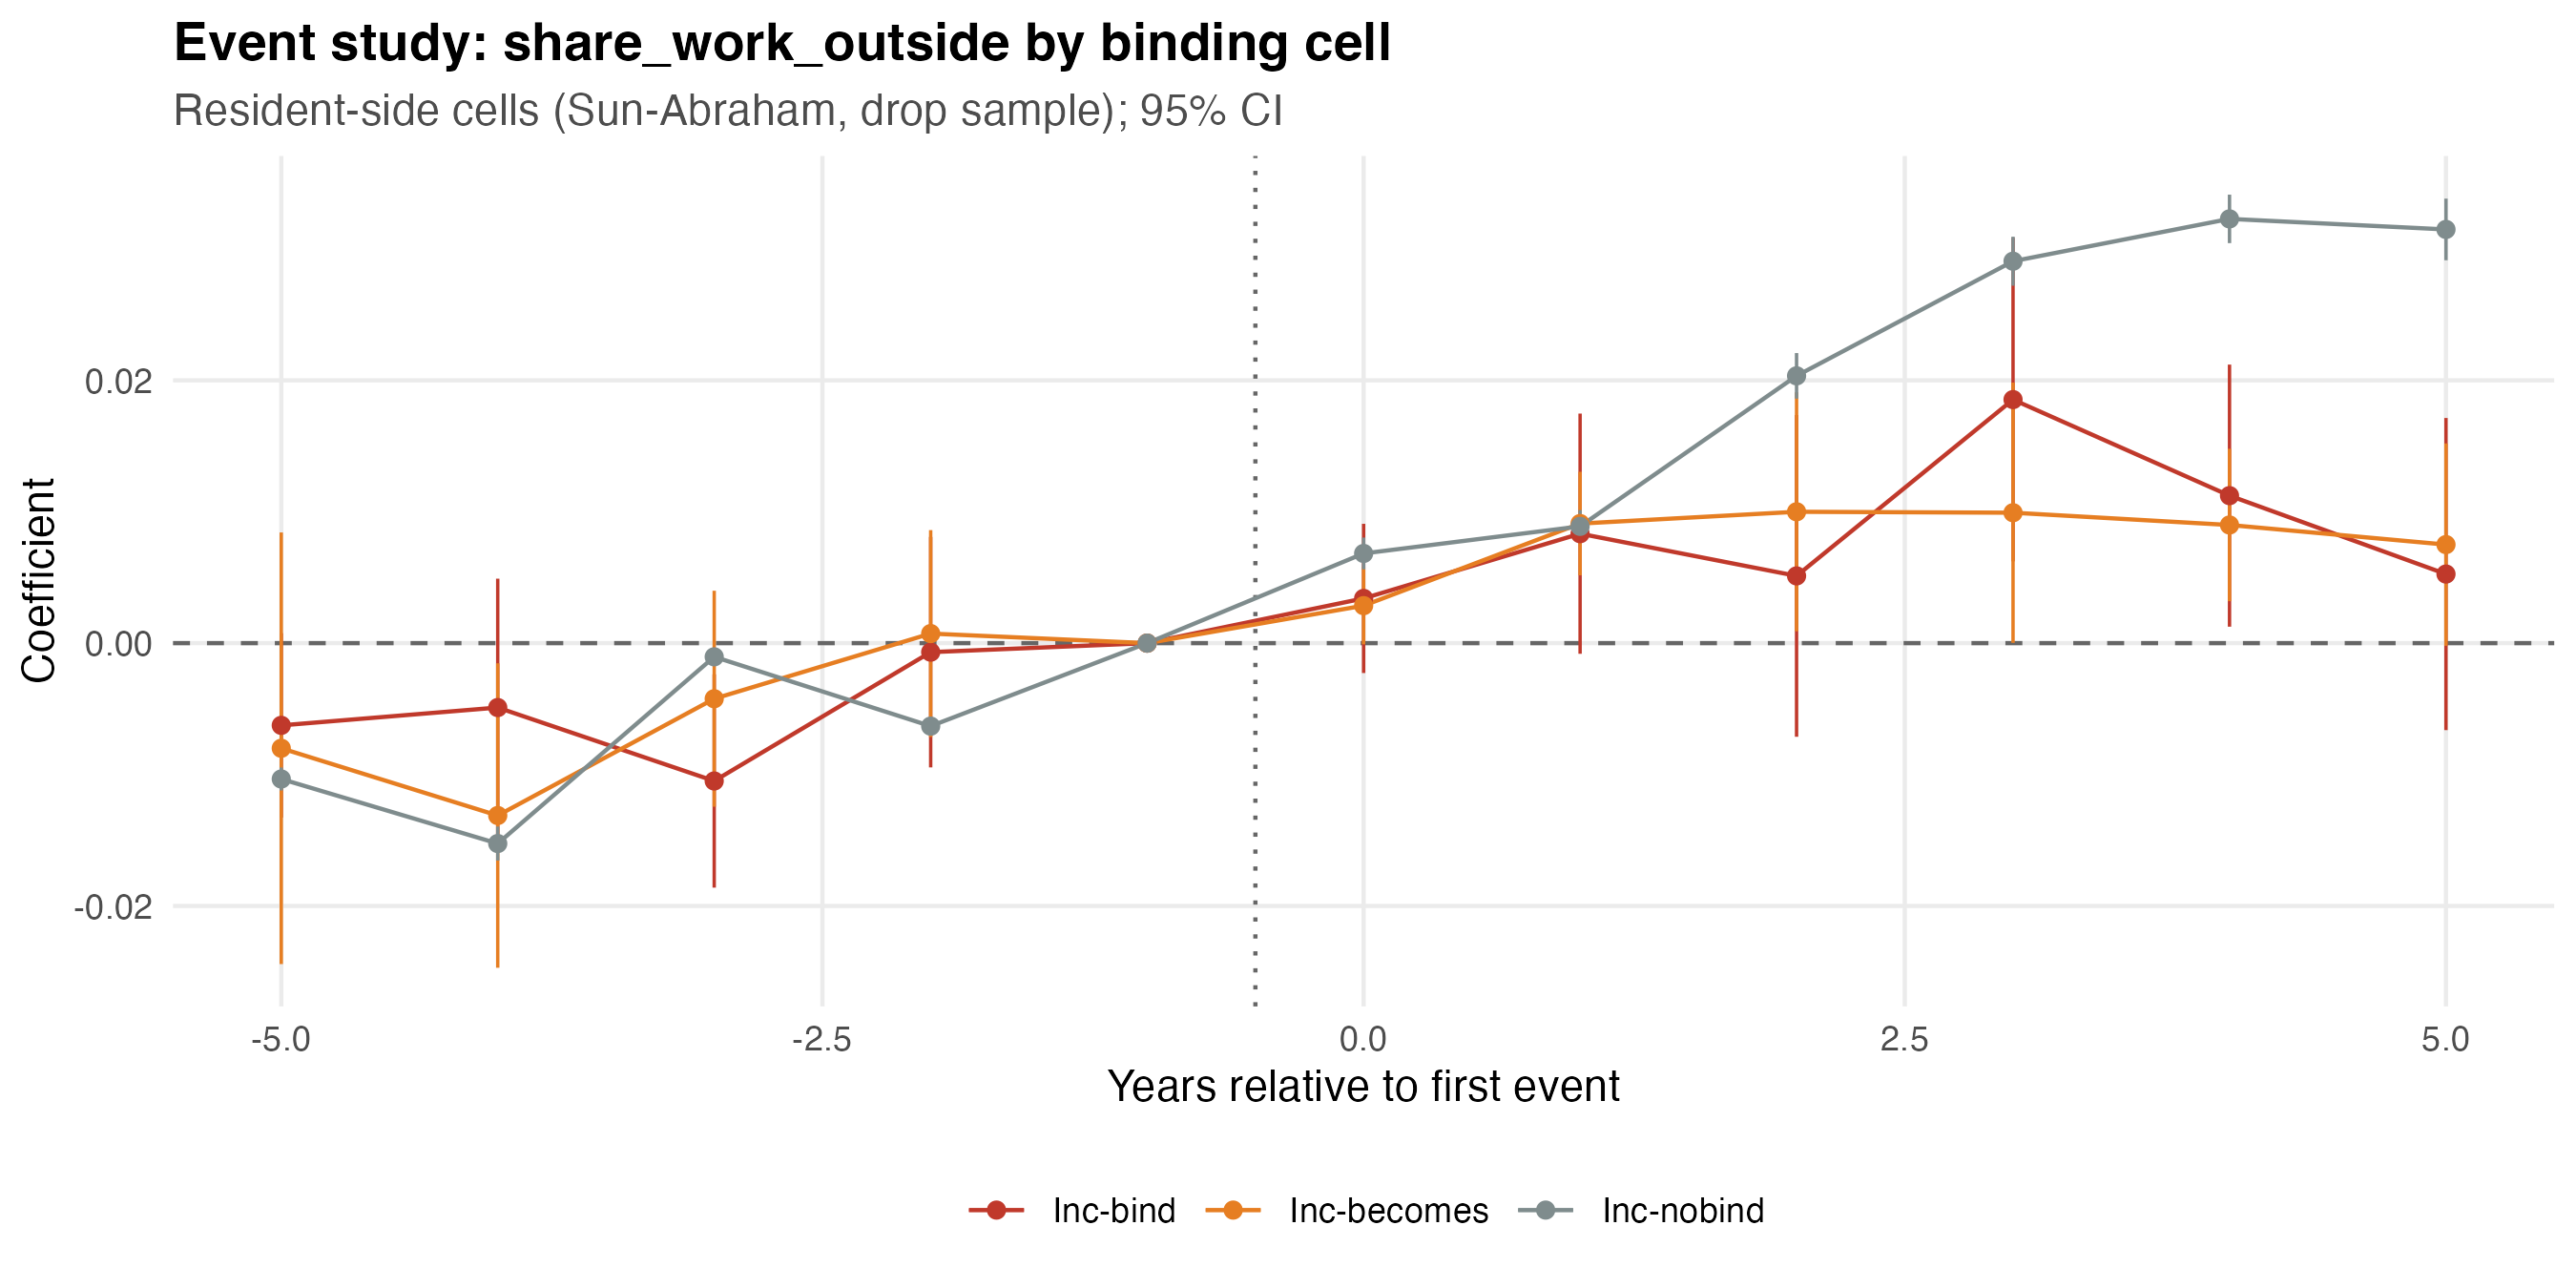
\includegraphics[width=0.85\textwidth]{unified_es_res_inc_share_work_outside.png}
        \vfill
        \footnotesize
        Share of residents commuting out. Inc-bind: $+3$pp;
        Inc-becomes intermediate. Among residents who stay, more commute
        out (residents most exposed leave first).
    \end{frame}
    %

    %
    \begin{frame}
    \fontfamily{cmr}
    \frametitle{Event Study: Dec Cells}
        \vfill
        \centering
        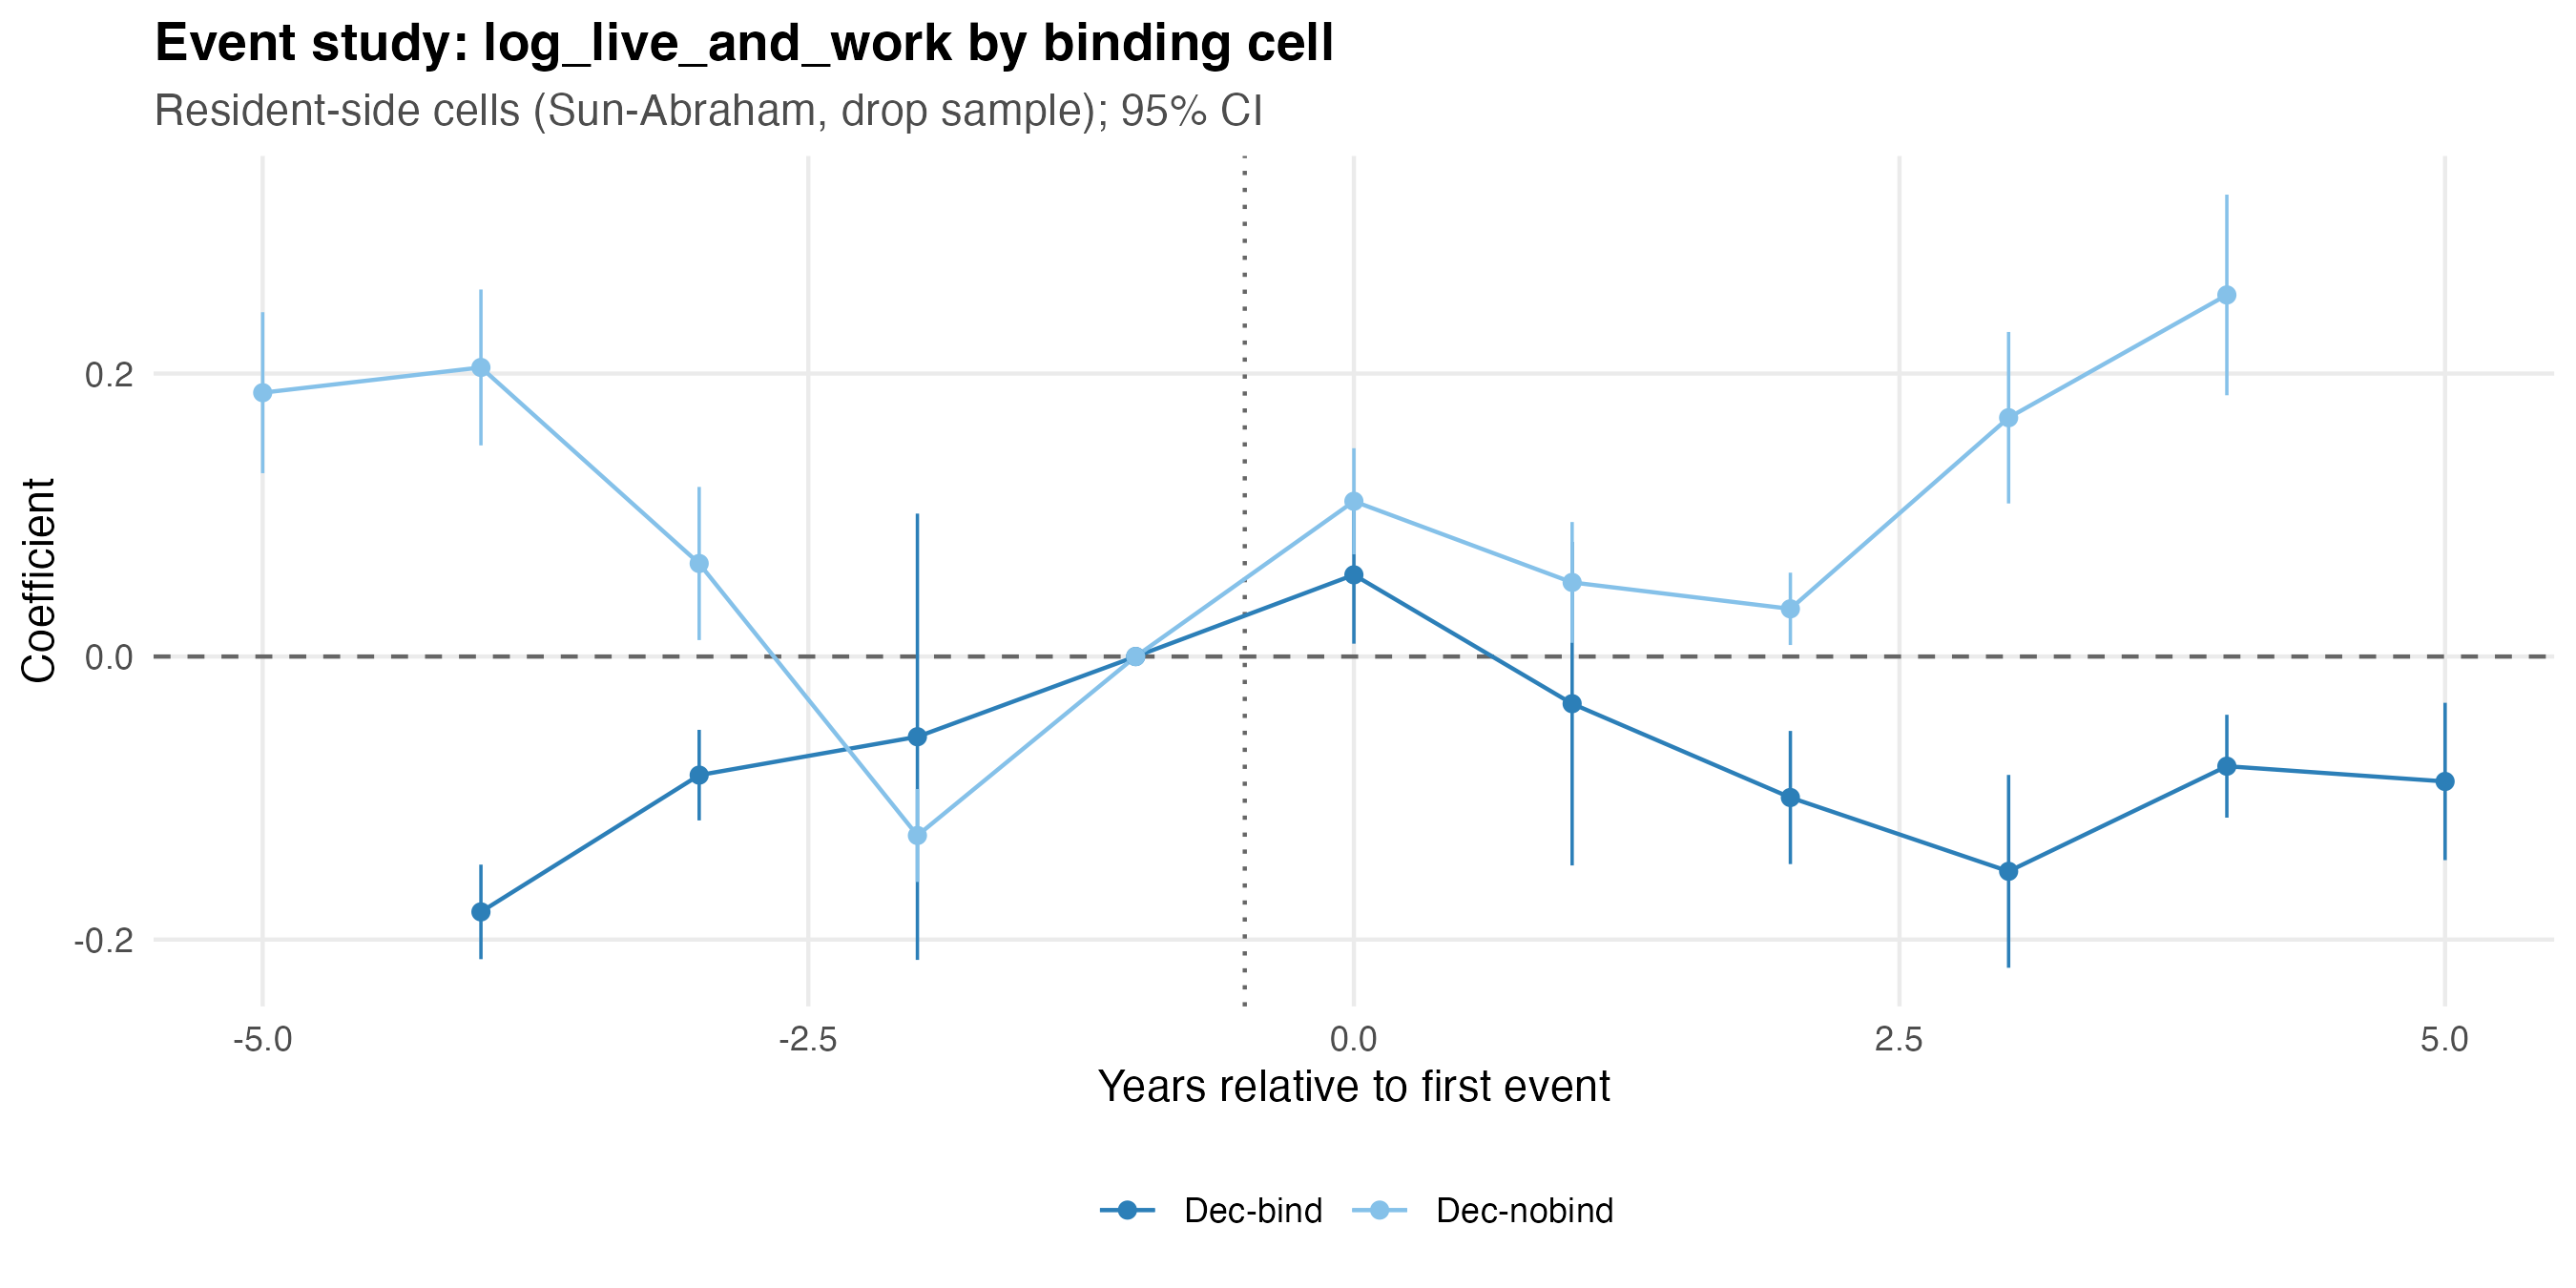
\includegraphics[width=0.85\textwidth]{unified_es_res_dec_log_live_and_work.png}
        \vfill
        \footnotesize
        Dec cells (11 + 15 munis). Direction broadly positive but
        underpowered. Cannot reject zero in either cell.
    \end{frame}
    %

%%%%%%%%%%%%%%%%%%%%%%%%%%%%%%%%%%%%%%%%%%%%%%%%%%%%%%
\section{Robustness}
%%%%%%%%%%%%%%%%%%%%%%%%%%%%%%%%%%%%%%%%%%%%%%%%%%%%%%

    %
    \begin{frame}
    \fontfamily{cmr}
    \frametitle{Robustness: Treatment Specification (Inc-bind, log\_live\_and\_work)}
        \centering
        \footnotesize
        \renewcommand{\arraystretch}{1.20}
        \setlength{\tabcolsep}{8pt}
        \begin{tabular}{lcc}
            \toprule
            Resident-side treatment & Inc-bind coef & $n$ Inc-bind munis \\
            \midrule
            Muni rate alone (one treatment)    & $-0.290^{***}$ & 40 \\
            Home stack (muni + SD combined)    & $-0.288^{***}$ & 101 \\
            Muni + SD separately (\textbf{headline}) & $\bm{-0.283^{***}}$ & 40 \\
            \bottomrule
        \end{tabular}
        \medskip

        \footnotesize
        \begin{itemize}\setlength{\itemsep}{0.04cm}
            \item Three treatment specifications, three nearly-identical
            Inc-bind muni effects ($-0.28$ to $-0.29$).
            \item The home-stack version captures 2.5$\times$ more
            ``binding-flip'' munis (101 vs 40) but the per-pp coefficient
            is essentially unchanged.
            \item \textbf{Result is robust to whether resident side is
            treated as one combined dose or decomposed.} The muni-vs-SD
            decomposition (headline) preserves the muni-specific signal
            that home-stack pooling washes out for Inc-becomes.
        \end{itemize}
    \end{frame}
    %

    %
    \begin{frame}
    \fontfamily{cmr}
    \frametitle{Robustness Across Samples (Inc-bind, log\_live\_and\_work)}
        \centering
        \footnotesize
        \renewcommand{\arraystretch}{1.20}
        \setlength{\tabcolsep}{8pt}
        \begin{tabular}{lccc}
            \toprule
            Estimator & strict & filled & drop \\
            \midrule
            Q2 TWFE pooled       & $-0.238$ & $-0.238$ & $-0.238$ \\
            Single-event TWFE    & $-0.157$ & $-0.157$ & $-0.157$ \\
            Stacked binary       & $-0.086$ & $-0.086$ & $-0.086$ \\
            Stacked continuous   & $-0.290$ & $-0.289$ & $-0.290$ \\
            \bottomrule
        \end{tabular}
        \medskip

        \footnotesize
        Coefficients are stable across the three samples
        (strict / statute-anchored fill / drop-incomplete). Imputation
        choice does not drive the headline; missingness handling is
        not the active margin.
    \end{frame}
    %

    %
    \begin{frame}
    \fontfamily{cmr}
    \frametitle{The Placebo Test: Inc-nobind Across Estimators}
        \centering
        \footnotesize
        \renewcommand{\arraystretch}{1.20}
        \setlength{\tabcolsep}{8pt}
        \begin{tabular}{lccc}
            \toprule
            & log(live\_and\_work) & log(total\_residents) & share\_live\_in \\
            \midrule
            Q2 TWFE pooled        & $-0.089^{**}$ & $+0.073$  & $-0.005$ \\
            Single-event TWFE     & $-0.078$      & $+0.071$  & $-0.005$ \\
            Stacked binary        & $-0.022$      & $+0.041$  & $+0.001$ \\
            Stacked continuous    & $-0.081$      & $+0.066$  & $-0.007$ \\
            DCDH                  & $-0.008$      & ---       & --- \\
            \bottomrule
        \end{tabular}
        \medskip

        \footnotesize
        \alert{Inc-nobind} = rate up but bill never moves.
        Across every estimator, level outcomes are within noise of zero.
        Q2 TWFE pooled is the only spec to reach 10\% on log(live\_and\_work)
        --- the spec most contaminated by negative weighting.
        \textbf{Bottom line:} when the rule says "no bill change,"
        we measure no behavioral change.
    \end{frame}
    %

    %
    \begin{frame}
    \fontfamily{cmr}
    \frametitle{Asymmetry: Inc Cells $>$ |Dec Cells|}
        \footnotesize
        Move costs predict Inc effects $>$ |Dec effects|.
        Data are consistent but Dec cells are underpowered:
        \medskip
        \scriptsize
        \renewcommand{\arraystretch}{1.20}
        \setlength{\tabcolsep}{8pt}
        \begin{tabular}{lccc}
            \toprule
            Outcome & Inc-bind ($n$=40) & Dec-bind ($n$=11) & Symmetric? \\
            \midrule
            log(live\_and\_work)  & $-0.290^{***}$ & $-0.284$ (insig) & ambiguous \\
            log(total\_residents) & $-0.121^{***}$ & $+0.169$ (insig) & sign reverses but noisy \\
            share\_work\_outside  & $+0.034^{**}$  & $-0.002$ (insig) & consistent with asymmetry \\
            \bottomrule
        \end{tabular}
        \medskip
        \footnotesize
        Decreases-binding has only 11 munis. Direction-of-sign tests are
        low-power. Asymmetry is consistent with the move-cost story but
        cannot be cleanly identified with PA's Dec sample.
    \end{frame}
    %

%%%%%%%%%%%%%%%%%%%%%%%%%%%%%%%%%%%%%%%%%%%%%%%%%%%%%%
\section{Conclusion}
%%%%%%%%%%%%%%%%%%%%%%%%%%%%%%%%%%%%%%%%%%%%%%%%%%%%%%

    %
    \begin{frame}
    \fontfamily{cmr}
    \frametitle{What This Design Replaces}
        \footnotesize
        The unified model subsumes three earlier framings into a single regression:
        \medskip
        \begin{itemize}\setlength{\itemsep}{0.05cm}
            \item \textbf{Block A / B / C separate sections}: collapsed
            into outcome rows of one regression.
            Block A's ``log(Resident workers)'' is now the Inc-bind column on
            \texttt{log\_live\_and\_work}; Block C's
            ``log(Residents employed)'' is the Inc-bind column on
            \texttt{log\_total\_residents}.
            \item \textbf{Piecewise pair-flow model}: cousub-pair regression
            with binding-state transitions. Saturated by pair FE; aggregate null.
            Replaced by the binding decomposition at the muni level, where
            sample sizes are tractable and signal survives.
            \item \textbf{Q3 asymmetry section}: the Inc/Dec direction split
            is now a within-design dimension of the cell taxonomy.
        \end{itemize}
    \end{frame}
    %

    %
    \begin{frame}
    \fontfamily{cmr}
    \frametitle{Summary}
        \begin{enumerate}\setlength{\itemsep}{0.08cm}\footnotesize
            \item \textbf{Causal effect on residential sorting: yes.}
            Muni Inc-bind cell, every estimator: consistent negative on
            log(live\_and\_work) and log(total\_residents); positive on
            share commuting out.
            \item \textbf{Within-design placebo passes.} Muni Inc-nobind
            cell --- rate hike that doesn't move the bill --- null behavior
            on every level outcome. The institutional rule, not generic
            confounding, identifies the response.
            \item \textbf{Three rates, three populations.} Muni rate
            moves residents (live-and-work, total residents); SD rate
            moves no one; nonres rate moves in-commuters.
            SD doesn't sort \emph{even within the binding decomposition} ---
            stronger version of the prior block-level-LODES finding.
            \item \textbf{Magnitude (stacked continuous, headline).}
            1pp \emph{muni}-rate hike when home binds $\Rightarrow$
            $-28\%$ live-and-work, $-12\%$ total residents,
            $+3.3$pp share commuting out.
            \item \textbf{Robust to treatment specification.} Muni-only,
            home-stack combined, and muni+SD-separate all give
            $-0.28$ to $-0.29$ on Inc-bind / log(live\_and\_work).
        \end{enumerate}
    \end{frame}
    %

    %
    \begin{frame}
    \fontfamily{cmr}
    \frametitle{Next Steps}
        \footnotesize
        \begin{itemize}\setlength{\itemsep}{0.05cm}
            \item \textbf{Add \texttt{share\_intergov} control} (intergov
            revenue / total revenue) --- silently dropped from later
            scripts. Re-run unified spec with full controls.
            \item \textbf{Industry decomposition} (issue \#2): pull WAC files
            for NAICS-supersector breakdowns to test the
            local-services-demand mechanism.
            \item \textbf{Spatial spillovers} (issue \#3): where do leavers go?
            Neighbor-shock spec on the residence-side outcomes.
            \item \textbf{Imputation diagnostic}: empirical share of
            muni-years where reported \texttt{nonres == resident\_eit}
            documents the statute-anchored fill (footnote).
            \item \textbf{Dec cells underpowered}: 11--15 munis per Dec cell.
            Multi-state extension would help.
            \item \textbf{Welfare}: combine $-0.29$ behavioral elasticity
            with $+0.67$ revenue elasticity for MEB / Laffer-curve location.
        \end{itemize}
    \end{frame}
    %

    %
    \begin{frame}
    \fontfamily{cmr}
    \frametitle{Thank You}
        \centering
        \vfill
        \Large Questions?
        \vfill
        \normalsize
        \texttt{hocke069@umn.edu} \\
        \small github.com/MatthewHockert/local-income-tax-migration
        \vfill
    \end{frame}
    %

\end{document}
